%; whizzy -pdf
\documentclass[11pt,a4paper]{article}
\usepackage[utf8]{inputenc}
%\usepackage[T1]{fontenc}
%\usepackage[swedish]{babel}
%\usepackage[us]{babel}

\usepackage[usenames,dvipsnames]{color}
\usepackage{graphicx}
\usepackage{subfigure}
\usepackage{floatflt}
\usepackage{wrapfig}

\usepackage{tikz}
\usepackage{bbding}

\usepackage{comment}

\usepackage{amssymb,amsmath}
\usepackage[pdftex,colorlinks=true,pdfstartview=FitV,
linkcolor=black,citecolor=RoyalBlue,urlcolor=RoyalBlue]{hyperref}

\setlength{\parindent}{0cm}
\setlength{\parskip}{0.3cm}

%\newcommand{\hawk}[1]{\texttt{#1}}
\newcommand{\hawk}[1]{\textsc{#1}}
\newcommand{\program}[1]{\textsc{#1}}
\newcommand{\com}[1]{\texttt{#1}}

\definecolor{gray}{rgb}{0.8,0.8,0.8}
\newcounter{exampleCount}

\newcommand{\example}[2]{
\refstepcounter{exampleCount}
\begin{tikzpicture}
\node[fill=gray, rounded corners=0.5cm]{

\hspace{0.2cm}\parbox{0.95\textwidth}{\vspace{0.1cm}\hspace{0.5cm}{\bf Example \arabic{exampleCount}: #1}\vspace{0.1cm}\hrule \vspace{0.3cm}
  #2
  \vspace{0.2cm}\hrule \vspace{0.3cm} }\hspace{0.2cm}
};
\end{tikzpicture}
}


\begin{document}
\begin{center}
  {\Huge \hawk{Hawk}}\\\vspace{0.3cm}
  {\Large Users Guide}\\\vspace{1cm}
\end{center}
\tableofcontents
\section{Introduction}
\subsection{What is Hawk?}
\hawk{Hawk} is a collection of command-line tools made to reconstruct objects from their diffraction patterns. The methods implemented in \hawk{Hawk} makes it suitable for analyzing diffraction patterns from single particles and not from, for example, crystalls. In addition to the command-line tools there is a graphical user interface (GUI), called \hawk{HawkGUI}, that can be used to controll some of the command-line tools in a more intuitive way. In later versions of \hawk{Hawk}, the GUI also implements some functions that are not available from the command-line. For this reason we suggest any user of \hawk{Hawk} to mainly use the GUI and only resort to the command-line tools for tasks not yet implemented in the GUI.

\subsection{How to use this document}
Read it!

\section{Preparing an image and image formats}
The image format used in \hawk{Hawk} contains a lot of information in addition to simple image, like for example what part of the image contains data and what doesn't. Therefore, any image to be used by hawk needs to be pre-processed into \hawk{Hawk's} \com{.h5} format. This process is not yet implemented in \hawk{HawkGUI} and therefore always has to be done from the command-line.

\subsection{The \com{.h5} format}
The file format used by \hawk{Hawk} is based on the \program{HDF5} format. It contains an image that can be complex or real and a binary mask that tells the programs what pixels that contain data and what pixels that, for example, was covered by the back-stop. It also holds information about where the center of the image is, what wavelength was used and what the distance from the detector to the interaction region was.

Images can be converted from \com{.tiff} files by using the program \hawk{tiff2h5}. For a list of options available for  this program (and most others in \hawk{Hawk} you can use \com{tiff2h5 -h}. The options \com{Input file}, \com{Output file}, \com{Distance to detector}, \com{Pixel size} and \com{Wavelength} has to be specified. If you do not have acces to all of the latter three you can input arbitrary values but be aware that calculations of sizes and distances rely on these numbers and will therefore be faulty.

\subsection{\hawk{process\_image}}
In the previous section we converted the image to \com{.h5} to be readable by \hawk{Hawk}. It's not yet ready for beeing used for a reconstruction though. The program we will use to prepare the image is called \hawk{process\_image} and as usual a complete list of options is available by entering \com{process\_image -h}. Here we will describe the options that any user is likely to use.

\textbf{Input file (-i) \& Output file (-o):} The input file should be the output from the \hawk{tiff2h5} program and be of type \com{.h5}. The output file should also be of type \com{.h5} and is ready to be used for reconstructing.e

\textbf{Downsample by x times (-a):} If the image is very big, reconstructing can be very slow. If this is the case we can choose to scale down the image. The downsampling value should be a positive integer and it tells the program with what factor the image should be scaled down. For example an 1024x1024 pixel images downsampled by a factor of 4 will result in an 256x256 pixel image.

\textbf{Mask to mask out pixels (-m):} This can be any image readable to \hawk{Hawk} (\com{.h5}, \com{.tiff}, \com{.png}) and contains zero values (black) at points where we have no data. The simplest way to produce a mask is to use any image manipulation program, for example \program{The GIMP}, to fill in the bad regions, see \ref{fig:draw_mask}.
\begin{figure}
\centering
\mbox{\hspace{-0.1\textwidth}\subfigure[Mask backstop]
            {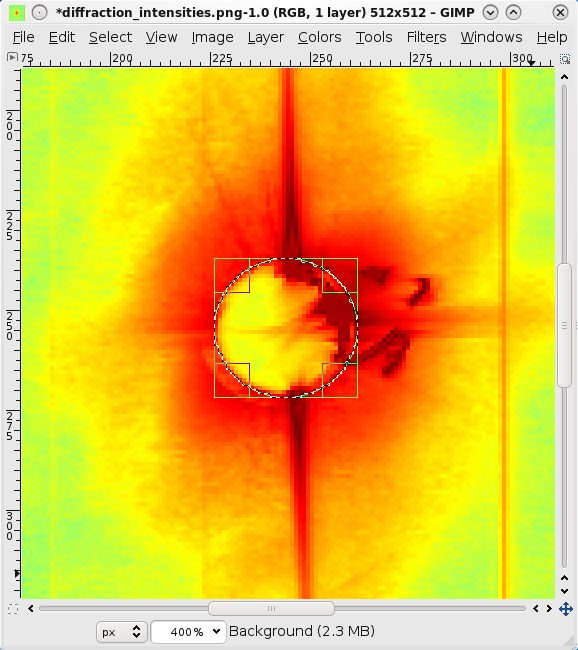
\includegraphics[width=0.4\textwidth]{Images/Remove_mask/beamstop1.png}\label{fig:mask1}}
  \subfigure[Mask other noise]
            {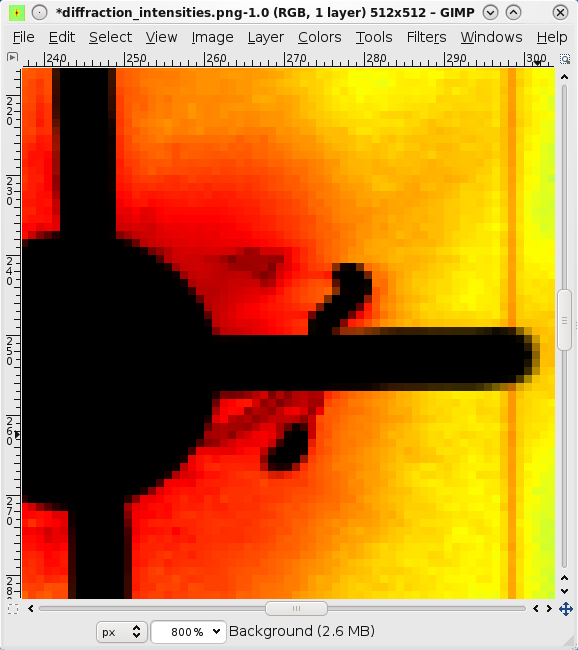
\includegraphics[width=0.4\textwidth]{Images/Remove_mask/small.png}\label{fig:mask2}}
  \subfigure[Missing columns]
            {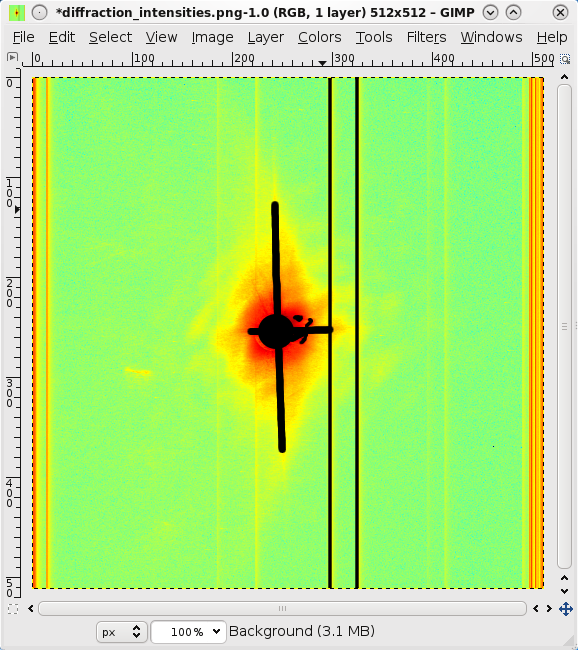
\includegraphics[width=0.4\textwidth]{Images/Remove_mask/stripes.png}\label{fig:mask3}}}
\mbox{\hspace{-0.1\textwidth}\subfigure[Final mask]
            {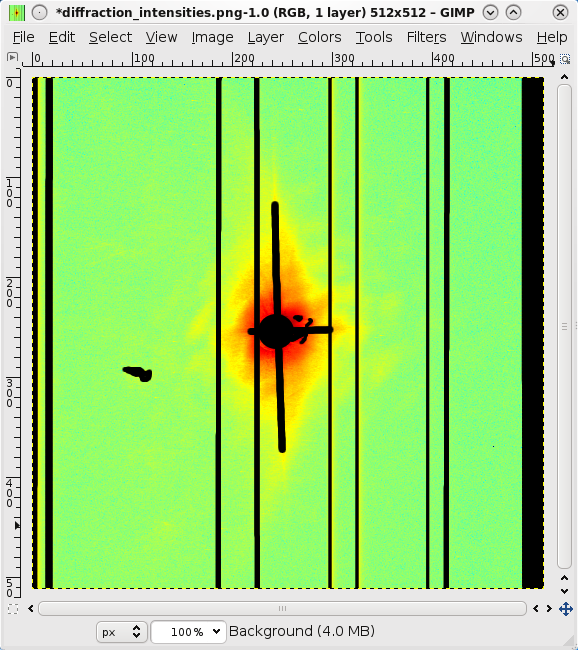
\includegraphics[width=0.4\textwidth]{Images/Remove_mask/all.png}\label{fig:mask4}}
  \subfigure[Select by color]
            {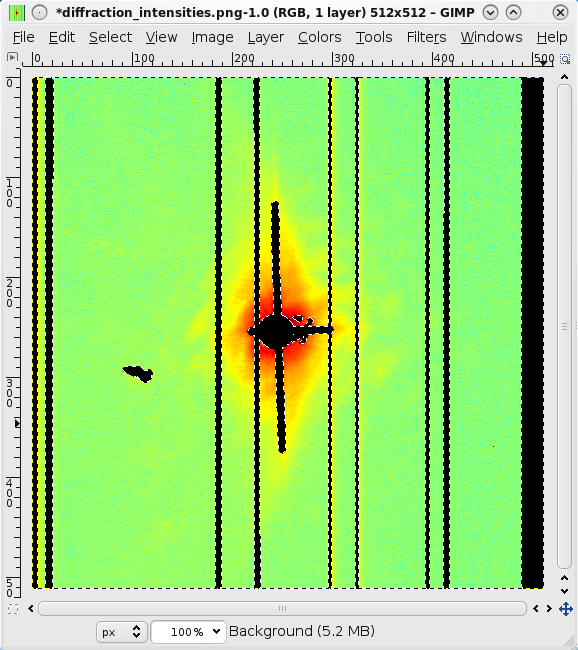
\includegraphics[width=0.4\textwidth]{Images/Remove_mask/select.png}\label{fig:mask5}}
  \subfigure[Finished]
            {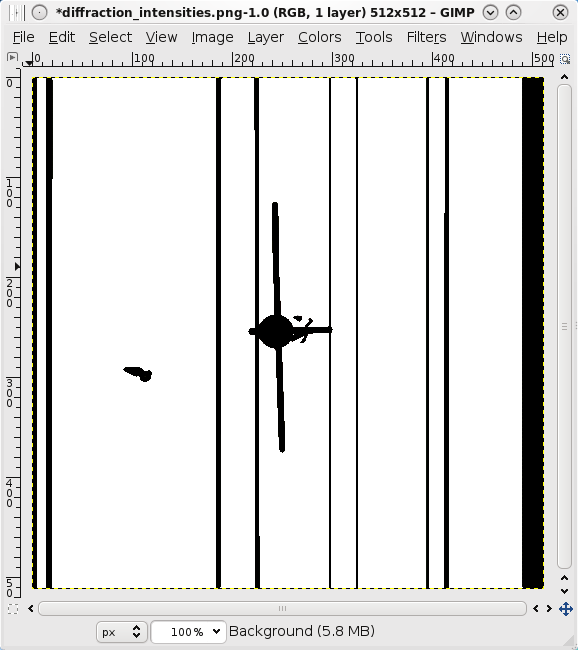
\includegraphics[width=0.4\textwidth]{Images/Remove_mask/final.png}\label{fig:mask6}}}
  \caption{\subref{fig:mask1} We start the masking by placing a selection over the backstop and filling it with black. \subref{fig:mask2} We then continue to draw over the features that are not part of the diffraction pattern. \subref{fig:mask3} In this image the detector gave us some full columns of bad values, we mask those out as well. \subref{fig:mask4} We have now masked out all the areas that doesn't contain diffraction data. \subref{fig:mask5} We then use the ``select by color'' tool in \program{GIMP} to select all the black parts. \subref{fig:mask6} The last step is to invert the selection and fill it with white. The mask is now done and can be saved in \com{.png} format.}
  \label{fig:draw_mask}
\end{figure}

\textbf{Maximum resolution to use in pixels (-r):} This option let's you crop the data at a specified number of pixels from the center. This is useful when the diffraction data doesn't stretch all the way out to the edge of the detector.

\textbf{User set image center (-c):} \hawk{process\_image} automatically finds the center of the image so typically this option is not needed. The center is found by convoluting the image with itself and searching for the maximum. Sometimes, especially if the image is non centro-symmetric (does not obey friedel symmetry) this algorithm can fail. When this happens the user can instead provide the center by this option. The syntax is \com{-c <center\_x>x<center\_y>} so if the center is at $x = 451$ pixels and $y = 518$ pixels the option should be passed as \com{-c 451x519}.

\textbf{Background level of the detector (-g):} This option allows the user to subtract a constant value from the image. By examining, for example the minimas between fringes the image, such a constant can sometimes be determined.

\example{\hawk{Process image}}{\label{ex:process_image}
  With the command \com{process\_image \--i image.h5 \--o processed.h5 \--m mask.h5 \--a 2} the $1024$x$1024$ pixel image, \com{image.h5}, will be processed, it will be downsampled to $512$x$512$ pixels and the mask $mask.h5$ will be applied. The result will then be saved as \com{processed.h5}}

\section{The Graphical User Interface}
When opening the \hawk{HawkGUI} you are met by the screen displayed in \ref{fig:GUIstart}
\begin{figure}
  \hspace{-0.2\textwidth}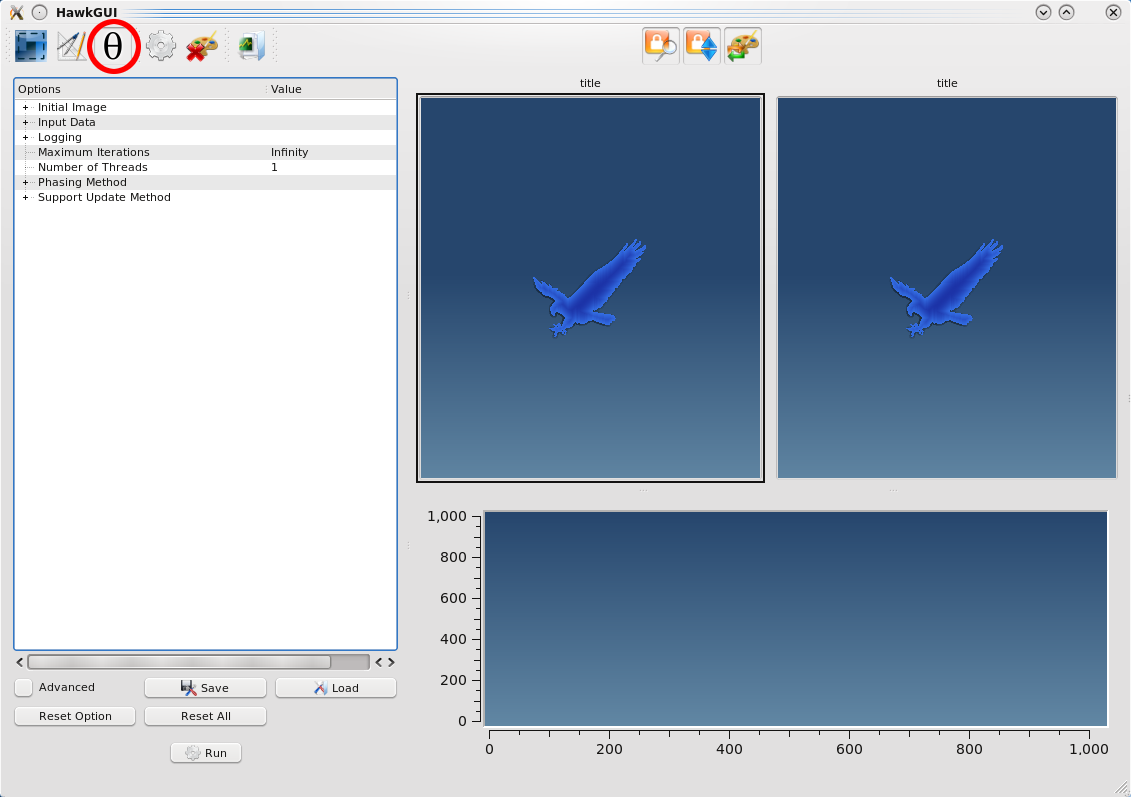
\includegraphics[width=1.4\textwidth]{Images/GUI/start.png}
  \caption{This is the starting screen of \hawk{HawkGUI}. The pressed button in the menu-bar (marked by the red circle) shows us that we are in reconstruction mode.}
  \label{fig:GUIstart}
\end{figure}

\section{Reconstructing}
\subsection{Algorithm basics}
\hawk{Hawk} uses two sets of information to reconstruct the image. One set is the data recorded by the detector. We know that the diffraction pattern of the object must fit this data. That is, the amplitudes of the fourier transform of the reconstructed object must equal the experimental amplitudes. The other piece of information that is needed is the shape of the object, called the \emph{support}. The goal of the algorithm is then to find an image that satisfies both these constraints. A very simple algorithm to do this is to repeatedly project on the set of all images that satisy the support constaint and on the set that satisfy the amplitudes constaint, see figure \ref{fig:twosets}. The algorithms used in practice will be a slightly more involved byt they are all based around this basic idea.
\begin{figure}
  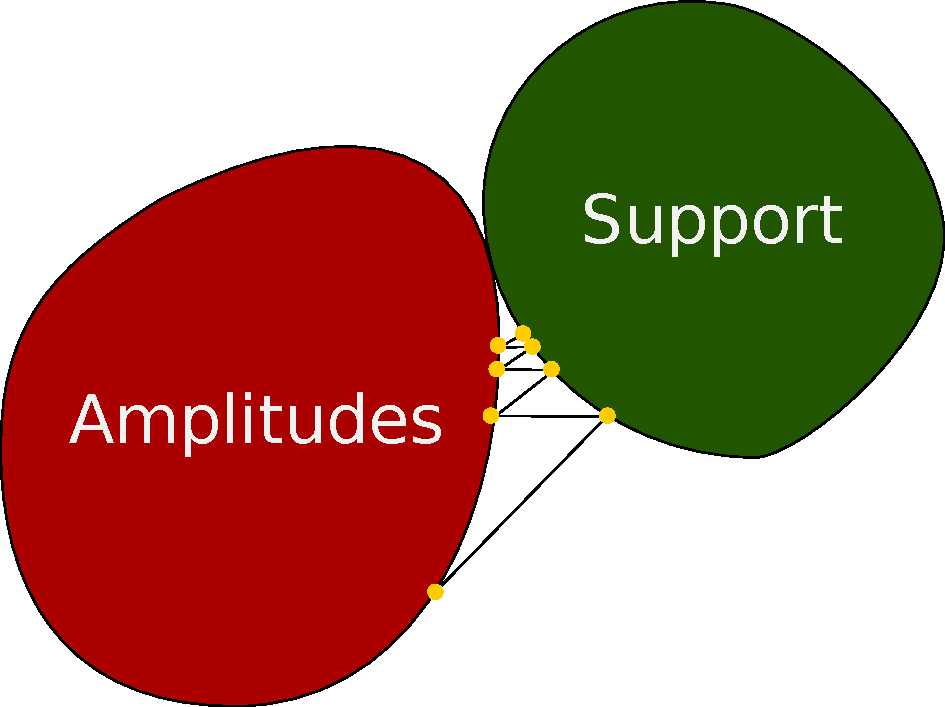
\includegraphics[width=0.9\textwidth]{Images/Convex_optimization/twosets.pdf}
  \caption{A reconstructed object must both fit the data (amplitude constraint) and have a certain size (support constraint). By repeatedly projecting on the closest image in each set that fulfill these constraint we will get closer and closer to the true image that fulfill both constraints.}
  \label{fig:twosets}
\end{figure}

One troublesome thing here is that we rarely know the shape of the object before reconstructing it. The workaround usually applied is to assume support that is sufficiently big to be guaranteed to be able to hold the object. As the reconstruction goes and our image of the object becomes better and better, this first guess can be improved. Unfortunatley, this approach has not been proven to work (and will not likely be so) but there is a large amount of cases where it has been empirically shown to work.

Another problem with the algorithm described above is that the sets are assumed to be \emph{convex}. When this is not the case there might be local stable points, or \emph{local minima} that will cause the algorithm to stagnate at a point that is not the true solution, see figure \ref{fig:twosets_nonconvex}.
\begin{figure}
  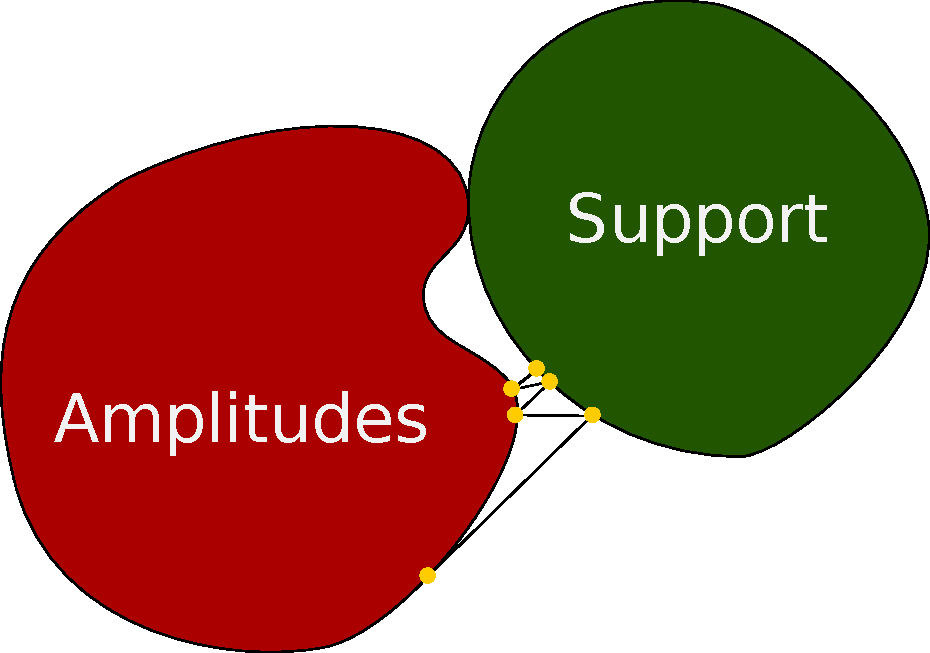
\includegraphics[width=0.9\textwidth]{Images/Convex_optimization/twosets_nonconvex.pdf}
  \caption{This figure shows what might happen when the sets are not convex. The algorithm has got stuck in a local minimum even though this is not the true cutting point of the sets.}
  \label{fig:twosets_nonconvex}
\end{figure}

The truth is that the set of support constrained images is a true convex set but the amplitudes constraint is not. Even thought the algorithms that are used in practice have some probability of escaping from local minimas, the solution is quite often not the true one. It is therefore usefull to run a reconstruction several times with different random starting guesses and thus increasing the probability of one of them to find the true minima.

\subsection{The programs}
The program that does the reconstruction is called \hawk{uwrapc} and can be called from the command-line. The convenient way to run it is however through the graphical user interface by simply clicking on the ``Run'' button. When this is done, the options entered in the list to the left will be read (more about them in the following sections). During the reconstructions, many files will be outputted and also displayed in the GUI. The most important ones are the \com{real\_space}, \com{support} and \com{fourier\_space}. The \com{real\_space} image shows the object at the current iteration. As mentioned before, the support is updated during the reconstruction, the \com{support} file gives you the current one. Last, the \com{fourier\_space} file shows the fourier transform of the object. All files are output both in the native \com{.h5} format which can store the full complex images, and the absolute values are outputted as a \com{.png} file for easy viewing.

\subsection{Essential parameters}
\subsubsection{Amplitudes file}
Here, the location of the imput amplitudes should be given. This should be the file outputted by \hawk{process\_image}. This file will be read but never overwritten. 

\subsubsection{Images output period}
This value is an integer that determines how often the current result is output to file. The images written to file are then read by the user interface so the output period will also be the update period of the on-line viewing in \hawk{HawkGUI}. Suitable update frequencies can vary from every 20 iterations up to more than every 1000 depending on the size of the images and the speed of the computer. Usually the number is choosen so that the program outputs an image every second or so.

\subsubsection{Log file}
\hawk{uwrapc} will output the current state of the reconstruction to a file. The information is then read and displayed by the GUI but the file can also be read by third-pary programs for a more thourough analysis or publication. More about the content of the file is available in section \ref{sec:logging}.

\subsubsection{Log output period}
This integer determines at what period the log file is updated. It can usually be choosen in the same way as the ``images output period''.

\subsubsection{Working directory}
All images written to file will be written to this directory.

\subsubsection{Maximum iterations}
This parameter specifies for how many iterations the reconstruction will run. Normaly when reconstructing we want to folow the progress of the reconstruction on-line and decide when to stop it on the fly. Therefore the standard value for this parameter is \com{Infinity}. When running multiple runs of the same reconstruction (see section \ref{sec:averaging}) this parameter becomes important.

\subsubsection{Number of threads}
When running \hawk{Hawk} on a computer with several CPU cores there is the possibility of using several cores for the reconstruction. This parameter specifies how many cores will be used.

If the machine is equipped with a modern NVIDIA graphics card, or graphical processing unit (GPU), this will be used for reconstructing with an order of magnitude speedup. This parameter will then be without effect.

\subsection{Phasing algorithm with parameters}
\subsubsection{Hybrid input output (HIO)}
This is the most common reconstruction algorithm used for single-particle diffraction images, and also the default in \hawk{Hawk}. The difference when compared to the algorithm described in figure \ref{fig:twosets} is that the projeciton on to the support set is replaced by a more complicated expression. The benefit is that the algorithm gains the ability to escape local minima, but might offcourse also escape the global minima if it is not a pure section of the two sets.

HIO takes one parameter, named $\beta$, that shoul always be in the range $1 > \beta > 0$, and can be thought of as the enery put into the system. A high $\beta$ value gives a ``jumpy'' algorithm and a high chance fo escaping from local minima. However, if the global minima is not very well defined it might not stay there. A low $\beta$ will on the other hand give a very slow algorithm that thougroly examines each local minima that it falls into and will need a lot of time to get up from the minima again.

For most reconstructions $\beta = 0.9$ is a good tradoff. Only if the output looks very caothic is it suggested to decrease the value to perhaps $0.8$.

When setting the value of $\beta$ in the GUI we get the dialog shown in \ref{fig:beta}. This advanced dialog lets the user specify a $\beta$ that changes during the reconstruction. It might for example be useful to start out with a high beta to make the algorithm cover a lot of the search space and then slowly decrease it to let it settle in a minimum. To edit the curve we can enter new conrol points by simply clicking somewhere in the figure, and we can move existing points by dragging them. Points can also be removed by right clicking. By double clicking on a point we bring up two boxes for exact specification of the x and y value. This is useful not only because it gives you perfect control but it also lets you put points outside the field of view of the figure. As we will see later, there are several other parameters that can be varied in this way using similair dialogs.
\begin{figure}
  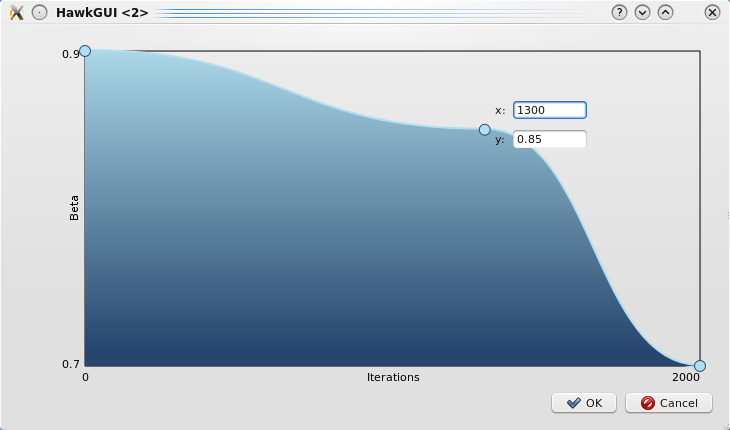
\includegraphics[width=\textwidth]{Images/GUI/beta.png}
  \caption{This dialog allows for a $\beta$ that changes during the progression of the reconstruction. In this example $\beta$ decreases slowly from $0.9$ to $0.85$ and then rapidly down to $0.7$. Existign points can be draged around and new ones can be created by clicking on an empty part of the plot. Points are deleted by right clicking and double clicking brings up the boxes for seting the exact value.}
  \label{fig:beta}
\end{figure}

\subsubsection{Relaxed averaged alternating reflections (RAAR)}
The relaxed averaged alternating reflections (RAAR) algorithm is another very good algorithm. It's behaviour differs from the HIO in that it is better in finding solutions if the starting guess is fairly close to it. HIO on the other hand is better at surveying a large search space for the solution. These guidelines are not very reliable, nor easy to use though. Therefore it's usually common to try both algorithms on any problem.

A particularly fruitful use of these two algorithms is to start by running HIO until the object shape is fairly close to our prior knowledge of the object. By then swiching to RAAR by using the last object and suport as input to another reconstruct, the reconstruction will find the best minimum close by. One word of coution that should be mentioned about this technique is that the result gets less reliable since we bias the result towards what we are expecting when we choose the breaking point of the HIO algorithm.

The RAAR algorithm also has in input parameter called $\beta$. This parameter has the inverse effect as the $\beta$ for HIO though, high values makes it unlikely for the algorithms to escape local (or global) minimas and low values makes it likely. The range is $1 > \beta > 0$ and a value of $0.9$ is reasonable.

\subsubsection{Difference map (diff\_map)}
Difference map is a newer algorithm that can be seen as a generalization of HIO since with a certain parameter selection it behaves exactly the same. Difference map takes two input variables $\gamma_1$ and $\gamma_2$. These are values between $0$ and $1$ and should are usually set to \emph{auto} with gives reasonable values.

This algorithm usually behaves similairly to HIO, sometimes better and sometimes worse so whenever HIO faies it might be good to try the difference map. In comparison to both HIO and RAAR this algorithm is slow, therefore it's seldom the first choise for any reconstruction.

\subsection{Support update algorithm}
Almost all reconstruction algorithms rely on a well-known support for convergence. For experimental data it is however very unlikely that the support is known. The common way of overcoming this problem is to start with a very big support and gradually decrease its size as the knowledge of the shape of the object becomes better. This section describes the parameters that are involved in support handling.

\subsubsection{Threshold}
When the support is updated using the threashold algorithm, every pixel in the current image of the object is compared to the highest pixel value. If it is higher than a user-specified threashold it becomes part of the new support, if it is lower it does not becom part of the support. See example \ref{ex:threshold}.

\example{Threshold}{\label{ex:threshold}
  If the threshold is set to $0.2$ and the maximum falue of the object in the current iteration is $24.3$ then every pixel with a value hither than $20$\% of that, or $4.86$, will become part of the new support.}

One problem that often occur when using this algorithm is that the support over-shrinks. If an unlycky reconstruction gives a support that is smaller than the actual object, even if it is only by one or a few pixels, the reconstruction usually shrinks the object and the support to a single spot.

\subsubsection{Decreasing area}
As a solution to the problem with the Threashold algorithm, the \emph{Decreasing area} algorithm was implemented. Here the risk of a shrinking support is avoided by using a fixed area instead. The area is given by the user in units of the whole field of view and the most intense pixels are choosen as parts of it. See example \ref{ex:area}.

\example{Decreasing area}{\label{ex:area}
  If the specified area is set to $0.01$ ($1$\%) and the image dimensions are $512$ x $512$ then the updated support will always have a size of $1$\% of the $262144$ pixels i. e. $2621$ pixels. The pixels are choosen to bee the most intense pixels in the object at the current itteration.}

The area is adjusted with in the same kind of dialog as in figure \ref{fig:beta}. This allows for the very useful technique of starting with a large area and let it slowly decrease to the true object area.

The algorithm can usually cope with an area that is a bit larger than the true one but not one that is smaller. A drawback compared to the threshold algorithm is that the area needs to be known. If it is not a  bit of trial and error is usually needed for finding the propper area, but this is usually the case for the threshold parameter as when using that algorithm.

\subsubsection{Innerloop iterations}
As mentioned above, the support is not updated every iteration. The algorithm is given some time in between updates to equilibrate at the new support. The frequency of the update is determined by the user by setting the \com{innerloop iterations} variable. The default value is $20$ and there is only rarely a reason to change it.

\subsubsection{Blur}
It is usually problematic if the support lacks pixels that should actually be part of the object, even if there is only a single pixel missing. The cause for pixels lacking can be since the area is set too small or the threshold is too agressive but can also just be an effect of random fluctuations. The last effect can be helped by smoothening the object before calculating the support. This way, no single pixel will have a very large effect on the support. The drawback is instead that the support will not become very tight since the edbes of the object will be blured.

The best trade-off is usually to start by using a large blur to stop the support from fluctuating to much. When the reconstructed image becomes better and more stable, the fluctuations will become smaller and we can allow for a smaller ammount of blur. The default blur starts at 3 pixels and drops to 0.7 pixels during the reconstruction. What starting blur to choose can vary quite a lot depending on for example the quality of the data and the resolution. There are few general guidelines but as a rule of thumb can be said that if the threshold algorithm frequently shrinks to a dot, a larger blur is called for. The final blur should usually be keept at below one pixel, only if the theoretical resolution is larger than one pixel should larger final blurs be considered.

\subsubsection{Support image averaging}
Another way of limiting the problems with random fluctuations explained in the previous section is to average the image output from several iterations and use this combined image to calculate the new support. This can be done by seting the \com{Support image averaging} parameter to a value higher than one.

\subsubsection{Initial support}
The initial support can be specified directly by giving an image as input for the \com{Initial Support} variable. The normal case is however that this variable is not set and that a crude support is estimated from the autocorrelation function.

The initial support is selected in essentialy the same way as the later ones but is's selection method can be choosen independent. The algorithm for creating the support is choosen with the paramter \com{Autocorrelation Selection Algorithm} and can be set to either \com{threshold} or \com{area}. For each choice the value for the threshold or area can be set by the variable \com{Autocorrelation Threshold} or \com{Autocorrelation Area} respectivley. The blur applied to the autocorelation befor using it to create a support can also be set by the variable \com{Autocorrelation Blur Radius}.

\subsection{Starting point}
Will be written when the implementation is fixed.

\section{Averaging many reconstructions}
\label{sec:averaging}
Any reconstruction will be biased by its starting position and therefore any single reconstruction should not be trusted to any large degree. \hawk{Hawk} has a tool for runing multiple reconstructions and then another tool for averaging them.

The tool is a perl script with the name \com{repeat\_reconstruction.pl}. To use it we need a configuration file from \hawk{HawkGUI}. Anytime a reconstuction is started, all the options for the current reconstruction is saved in a file called \com{uwrapc.conf} in the current working directory. You can also save the options by using the ``Save'' button below the options field in the GUI.

The options file should be put in an empty directory and then the \com{repeat\_\-reconstruction.pl} script should be called from this directory. The script takes one argument and two more optional arguments. The first argument is the number of reconstructiosn that should be run. The second argument is the number of the first reconstruction, this is useful when you have already run a number of reconstructions but want to add more. The last argument specifies the number or processor cores that will be used.

\example{Repeat reconstruction}{\label{ex:repeat}
  The command \com{repeat\_reconstruction.pl 10 0 2} will run a  $10$ reconstructions each on $2$ cores, for a total of $20$ reconstuctions. The second argument means that the indexing will start at zero so the last reconstruction will be given the index $19$.
}

When run, the script will create a new directory for each reconstruction named by the index of this reconstruction. These directories will be used as the working directory for the respective reconstruction. 

Next step is to put all the reconstructions together by using the \hawk{prtf} program. This program reads many reconstructed images and creates an average. In adition to the average it also estimates the quality of the image by studying the differences between the reconstructions.

The input files should be the reconstructed objects, including the complex phase. These are found in the files \com{real\_space-final.h5} for the respective reconstruction. The images are translated relative to each other before averaging since the relative position is not coded for in the diffraction pattern but is an artifact from the algorithm. This fit also allows for the images to be mirrored around the center if this gives a better fit since the different between the true object and its centrosymmetric copy is not encoded for in the pattern either.

\begin{figure}
  \centering
  \subfigure[Original]{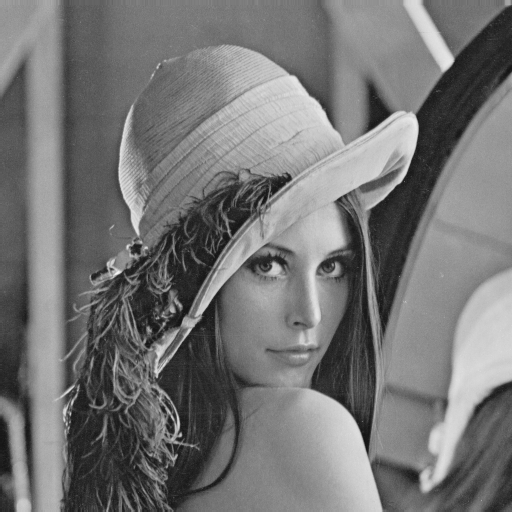
\includegraphics[width=0.4\textwidth]{Images/PRTF/lena.png}\label{fig:cent1}}
  \subfigure[Centrosymmetric copy]{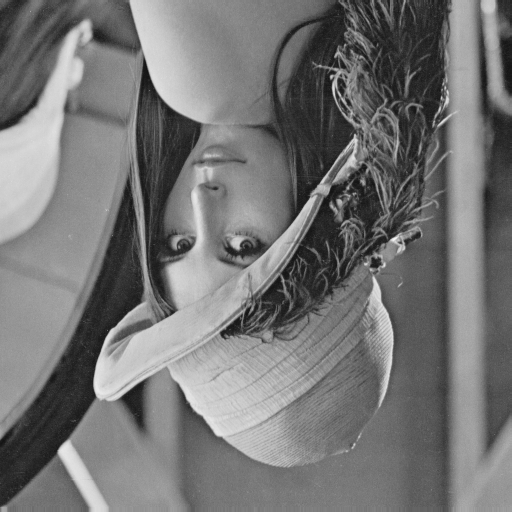
\includegraphics[width=0.4\textwidth]{Images/PRTF/lena_centrosymmetric.png}\label{fig:cent2}}
  \caption{This image shows an example of an image and its centrosymmetric copy. These two images are indistinguishable from their diffraction patterns alone.}
  \label{fig:cent}
\end{figure}

\begin{figure}
  \centering
  \subfigure[Image 1]{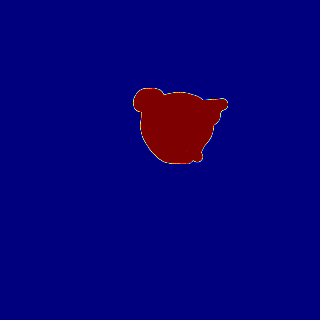
\includegraphics[width=0.4\textwidth]{Images/PRTF/foo/foo1_jet.png}\label{fig:foo1}}
  \subfigure[Image 2]{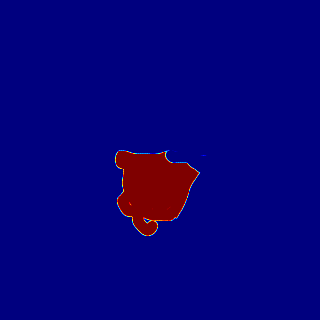
\includegraphics[width=0.4\textwidth]{Images/PRTF/foo/foo2_jet.png}\label{fig:foo2}}
  \subfigure[Image 3]{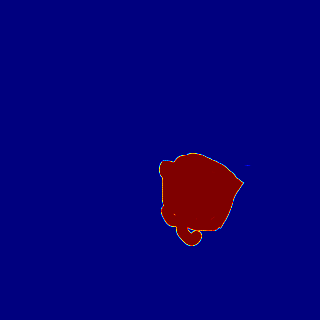
\includegraphics[width=0.4\textwidth]{Images/PRTF/foo/foo3_jet.png}\label{fig:foo3}}
  \subfigure[Image 4]{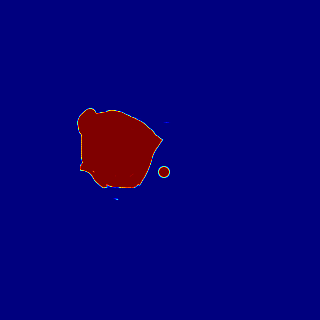
\includegraphics[width=0.4\textwidth]{Images/PRTF/foo/foo4_jet.png}\label{fig:foo4}}
  \subfigure[Average image]{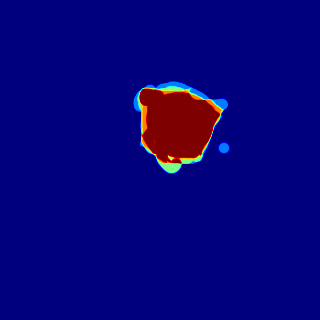
\includegraphics[width=0.4\textwidth]{Images/PRTF/foo/foo-avg_image.png}\label{fig:foo_average}}
  \subfigure[PRTF]{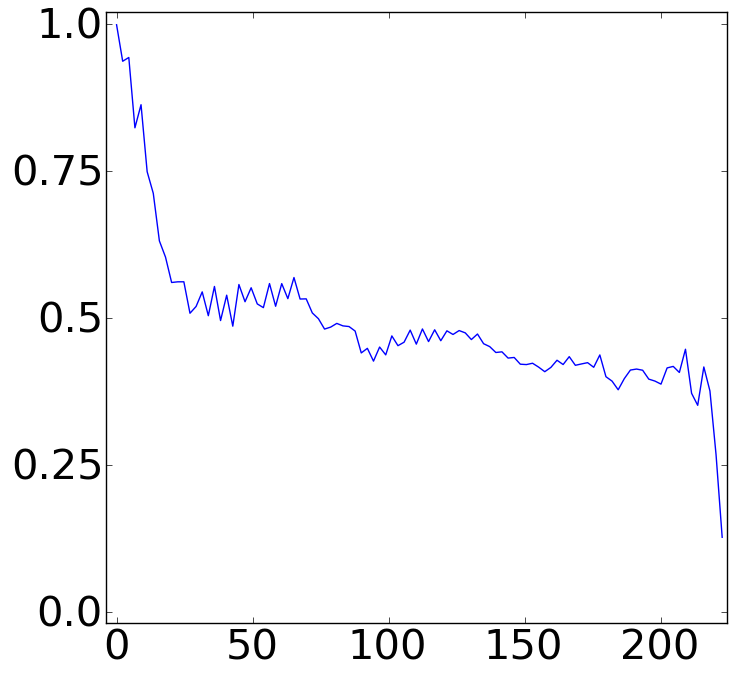
\includegraphics[width=0.4\textwidth]{Images/PRTF/foo/foo_prtf.png}\label{fig:foo_prtf}}
  \caption{Images \subref{fig:foo1} to \subref{fig:foo4} are averaged using \hawk{prtf}. The average image \subref{fig:foo_average} superimposes the objects even though they are translated with respect to each other. In \subref{fig:foo_prtf} we see the phase retrieval transfer function (PRTF). It passes through $e^{-\frac{1}{2}}$ at about pixel $210$ this tells us that our resolution is about $\frac{210}{320} = 1.52$ pixels where $320$ is the image dimension.}
  \label{fig:prtf}
\end{figure}

To estimate the resolution of the recovered image the \hawk{prtf} program calculates the phase retieval transfer function (PRTF), which has also given it's name to the tool. The PRTF is, for every pixel $i$ in diffraction space
\begin{equation}\label{equ:prtf}
  \mathrm{PRTF}_i = \frac{\left| \sum_n F_{in} \right|}{\sum_n \left| F_{in} \right|}
\end{equation}
where $F_{in}$ is the vale of the $i$th pixel in the $n$th reconstruction. Since all reconstructions originate in the same diffraction pattern, the absolute value of $F_{in}$ will be the same for all $n$. The phase might differ and for that reason the nominator in \ref{equ:prtf} can be smaller than the denominator. The more different the reconstructed objects are, the more different will the phases be and the smaller the value for the PRTF. The PRTF is therefore a measure of the quality of the reconstruction.

It is especially usefull to plot the radial average of the PRTF (see figure \ref{fig:foo_prtf}). This plot gives the quality of the reconstruction as a function of resolution. By convention, the resolution is defined by the resolution-shell where the radially averaged PRTF passes through $e^{-1} = 0.368$. An example of a run of \hawk{prtf} is shown in figure \ref{fig:prtf}.

When invoking \hawk{prtf} the first argument given is a prfix that is prepended to the filenames of all the outputted files. After this argument comes all the files that are used in the prtf. For example the PRTF in figure \ref{fig:prtf} was calculated by \com{prtf my\_prtf \-image1.h5 \-image2.h5 \-image3.h5 \-image4.h5}. 

The averaged image is saved to a file named \com{<prefix>-avg\_image.h5} and a \com{.png} copy is also saved. The PRTF function is outputted as \com{<prefix>-prtf.h5}. The radial average is saved in a text file named just \com{<prefix>} containing two columns. The first column contains the radius of each shell in pixels and the second contains the averaged PRTF.

\example{\hawk{PRTF}}{\label{ex:prtf}
  To average the output from example \ref{ex:repeat} wee need to input one file from each subdirectory . On a \program{linux} or \program{mac} machine this can be done by \com{prtf <prefix> */real\_space-final.h5}. The \com{*} will make sure that files named \com{real\_space-final.h5} in all subdirectories are included in the PRTF.
}

\section{Reconstructing on graphics cards}
On computers equipped with modern NVIDIA graphics-cards, reconstructions can be speed up by up to a factor of 100. What is needed is that the \program{CUDA} drivers (available from the NVIDIA homepage) are installed and that \program{CUDA}-support is turned on uppon when installing \hawk{Hawk}.

\begin{comment}
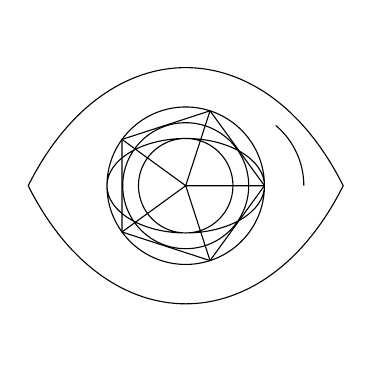
\begin{tikzpicture}
  \path (0,0) coordinate (origin);
  \path (0:1cm) coordinate (P0);
  \path (1*72:1cm) coordinate (P1);
  \path (2*72:1cm) coordinate (P2);
  \path (3*72:1cm) coordinate (P3);
  \path (4*72:1cm) coordinate (P4);

  \draw (P0) -- (P1) -- (P2) -- (P3) -- (P4) -- cycle;
  \draw (origin) rectangle (P0) (origin) -- (P1) (origin) -- (P2)
  (origin) -- (P3) (origin) -- (P4);
  \draw (0,0) circle (1cm) circle (0.8cm) circle (0.6cm) ellipse (1cm and 0.6cm);
  \draw (0:1.5cm) arc (0:50:1cm);
  \draw (-2,0) .. controls (-1,2) and (1,2) .. (2,0) .. controls (1,-2) and (-1,-2) .. (-2,0);
\end{tikzpicture}
\end{comment}

\section{Logging}\label{sec:logging}


\end{document}
